\documentclass[a4paper, 10pt, twoside, notitlepage]{article}
% idioma
\usepackage[spanish]{babel}
\usepackage[utf8x]{inputenc}
\usepackage{graphicx}

% graficos
%\usepackage[pdftex]{graphicx}
%\usepackage{wrapfig}

%\usepackage{listings}
%\lstset{language=C,basicstyle=\small}

%\usepackage{epic,eepic}
% estilo
\usepackage[footnotesize]{caption}
\usepackage[outer=2cm,inner=4cm,top=2cm,bottom=2cm]{geometry}
\usepackage{fancyhdr}
\usepackage{lipsum}

\usepackage{color,hyperref}
\definecolor{black}{rgb}{0.0,0.0,0.0}
\definecolor{darkblue}{rgb}{0.0,0.0,0.3}

\hypersetup{colorlinks,breaklinks,
            linkcolor=black,urlcolor=darkblue,
            anchorcolor=darkblue,citecolor=darkblue}

% matematica
\usepackage{amsmath} \usepackage{amsfonts} \usepackage{amssymb}

\title{\textbf{Trabajo Práctico 0:\\Ley de Amdahl} \\}

\author{ \\
         Ronnie Del Pino Cárdenas, \textit{Padrón 93575} \\
          \texttt{ delpinor@mail.com }       \\
          \texttt{ @delpinor }       \\
		  [2.5ex]
         Nombre Apellido, \textit{Padrón xxxxx}     \\
          \texttt{mail@mail.com}                      \\ 
		  [2.5ex]
		  Nombre Apellido, \textit{Padrón xxxxx}     \\
          \texttt{mail@mail.com}                      \\ 
		  [2.5ex]
		 \\
         \normalsize{2do. Cuatrimestre de 2019}            \\
         \normalsize{86.37 / 66.20 Organización de Computadoras $-$ Práctica Jueves} \\
         \normalsize{Facultad de Ingeniería, Universidad de Buenos Aires} 
       }

\date{}

\begin{document}

\maketitle
% \thispagestyle{empty}   % quita el número en la primer página

% \newpage
% Es un breve resumen de lo que vamos a leer con mayor profundidad en las secciones posteriores, tiene que resaltar lo más importante.
\begin{abstract}
El presente trabajo práctico nos permitió analizar la performance de un programa a partir de la implementación de una mejora sobre un módulo. Para su análisis se usaron herramientas de análisis de tiempos de ejecución y perfilado (\textbf{time  y gprof respectivamente}). Además se aplicaron los conocimientos adquirios sobre la Ley de Amdahl para el cálculo del SpeedUp.
\end{abstract}

% \tableofcontents
% 
% \newpage
% 

\pagestyle{fancy}
\fancyhead{}
\fancyfoot{}
\renewcommand{\sectionmark}[1]{\markright{\thesection\ #1}}
\renewcommand{\headrulewidth}{0.4pt}
%\renewcommand{\footrulewidth}{0.4pt}
\fancyhead[LE]{\nouppercase \rightmark}
\fancyhead[RE, LO]{\bf \thepage}
\fancyhead[RO]{\nouppercase \rightmark}
\fancyfoot[C]{ }
\maketitle
%genera el indice - compilar dos veces
\setcounter{page}{1}
% \tableofcontents
% \newpage

\parskip 7.2pt
%Distinto al resumen, se dice cual es el objetivo principal y se hace un resumen de cada parte que aparece a continuación. 
\section{Introducción}
A continuación se realizarán distintos procedimientos con motivo de  analizar el rendimiento de al menos dos implementaciones del algoritmo que llamamos "La hormiga artista". El analisis será llevado a cabo sobre un ambiente MIPS usando herramientas time y gprof del entorno de trabajo y la Ley de Amdahl.\\

La ley de Amdahl mide cuanto mejora o empeora un sistema al introducir mejoras en un sistema existente dependiendo de la frecuencia de utilización del elemento modificado.\\

\begin{equation}
 SpeedUp =\frac{1}{(1-Fm) + \frac{Fm}{Am}}
\end{equation}

Donde:\\

\textbf{Fm}: La fracción del tiempo de cálculo de la máquina original que pueda utilizarse para aprovechar la mejora.\\

\textbf{Am}: La optimización lograda por el modo de ejecución mejorado, es decir el factor de mejora que se ha introducido en el subsistema alterado.
%Una de las secciones más importantes del informe. Aquí se explaya todo lo realizado, problemas encontrados y soluciones propuestas con variantes y métricas.


\newpage

\section{Proceso de Compilación}

Se usó el archivo makefile provisto por el docente para generar los ejecutables tanto para crear los perfiles como así para conocer los tiempos de ejecución.\\

\begin{itemize} 
\item[] \textbf{make all}: Crea dos ejecutables tp0\_if y tp0\_tables.
 \item[] \textbf{make prof}: Crea dos ejecutables, tp0\_if\_pf y tp0\_tables\_pf.
\end{itemize}

Los dos primeros archivos fueron usados para medir los tiempos de ejecución usando la herramienta \textbf{time}, mientras que los subsiguientes para el perfilamiento usando la herramienta \textbf{gprof}.

Como primer paso ejecutamos las versión compilada para conocer el perfilado:
\scriptsize
\begin{verbatim}
#  ./tp0_tables_pf -g 10000x10000 -p RGBW -r LLLL -t $((1000 * 1000)) > /dev/null
\end{verbatim}
\normalsize

Una vez terminada la ejecución, usamos el siguiente comando para conocer el perfilado del programa:

\scriptsize
\begin{verbatim}
# gprof tp0_tables_pf gmon.out
\end{verbatim}
\normalsize

A continuación se muestran los resultados de perfilado plano para este caso de prueba donde se muestran en forma decreciente tomando el cuenta el porcentaje de tiempo total del programa que se dedicó a una función. Estos reportes muestran el tiempo de ejecuación y la cantidad de llamadas. 
\scriptsize
\begin{verbatim}
Each sample counts as 0.01 seconds.
  %   cumulative   self              self     total           
 time   seconds   seconds    calls   s/call   s/call  name    
 47.96      5.11     5.11        1     5.11     7.18  grid_out
 22.71      7.53     2.42        1     2.42     2.42  make_grid
 19.61      9.62     2.09 101000000     0.00     0.00  colour_at
  3.43      9.99     0.37  1000000     0.00     0.00  paint_at
  2.53     10.26     0.27        1     0.27     1.03  paint
  1.27     10.39     0.14  1000000     0.00     0.00  move_forward
  0.52     10.45     0.06  1000000     0.00     0.00  new_orientation
  0.47     10.50     0.05  1000000     0.00     0.00  rule_for_colour
  0.38     10.54     0.04  1000000     0.00     0.00  next_colour
  0.33     10.57     0.04   250000     0.00     0.00  step_west
  0.23     10.60     0.03   250000     0.00     0.00  step_east
  0.23     10.62     0.03   250000     0.00     0.00  step_north
  0.14     10.64     0.02                             frame_dummy
  0.09     10.65     0.01        1     0.01     0.01  make_palette
  0.09     10.66     0.01        1     0.01     0.01  make_rules
  0.05     10.66     0.01   250000     0.00     0.00  step_south
  0.00     10.66     0.00        9     0.00     0.00  get_colour
  0.00     10.66     0.00        5     0.00     0.00  xalloc
  0.00     10.66     0.00        2     0.00     0.00  atoui32
  0.00     10.66     0.00        1     0.00     0.00  destroy_grid
  0.00     10.66     0.00        1     0.00     0.00  destroy_palette
  0.00     10.66     0.00        1     0.00     0.00  make_ant
  0.00     10.66     0.00        1     0.00     0.00  make_grid_handler

\end{verbatim}
\normalsize
Es importante mencionar que en el reporte se aclara que el periodo de muestra es de 0.01 segundos por lo que un valor relativamente similar o menor a este se podría considerar no fiable.\\
\\
También se muestra otro de los reportes hechos por la herramientra donde se puede observar un grafo de llamadas. Este reporte es importamente ya que permite encontrar funciones que aunque ellas mismas no incurrieron en tiempos altos, llamarona a otras funciones que sí lo hicieron.

\scriptsize
\begin{verbatim}
granularity: each sample hit covers 2 byte(s) for 0.09% of 10.66 seconds

index % time    self  children    called     name
                                                 <spontaneous>
[1]     99.9    0.00   10.65                 main [1]
                5.11    2.07       1/1           grid_out [2]
                2.42    0.00       1/1           make_grid [3]
                0.27    0.76       1/1           paint [5]
                0.01    0.00       1/1           make_palette [15]
                0.01    0.00       1/1           make_rules [16]
                0.00    0.00       2/2           atoui32 [20]
                0.00    0.00       2/5           xalloc [19]
                0.00    0.00       1/9           get_colour [18]
                0.00    0.00       1/1           make_ant [23]
                0.00    0.00       1/1           destroy_palette [22]
                0.00    0.00       1/1           destroy_grid [21]
-----------------------------------------------
                5.11    2.07       1/1           main [1]
[2]     67.3    5.11    2.07       1         grid_out [2]
                2.07    0.00 100000000/101000000     colour_at [4]
-----------------------------------------------
                2.42    0.00       1/1           main [1]
[3]     22.7    2.42    0.00       1         make_grid [3]
                0.00    0.00       1/5           xalloc [19]
                0.00    0.00       1/1           make_grid_handler [24]
-----------------------------------------------
                0.02    0.00 1000000/101000000     paint [5]
                2.07    0.00 100000000/101000000     grid_out [2]
[4]     19.6    2.09    0.00 101000000         colour_at [4]
-----------------------------------------------
                0.27    0.76       1/1           main [1]
[5]      9.6    0.27    0.76       1         paint [5]
                0.37    0.00 1000000/1000000     paint_at [6]
                0.14    0.09 1000000/1000000     move_forward [7]
                0.06    0.00 1000000/1000000     new_orientation [8]
                0.05    0.00 1000000/1000000     rule_for_colour [9]
                0.04    0.00 1000000/1000000     next_colour [10]
                0.02    0.00 1000000/101000000     colour_at [4]
-----------------------------------------------
                0.37    0.00 1000000/1000000     paint [5]
[6]      3.4    0.37    0.00 1000000         paint_at [6]
-----------------------------------------------
                0.14    0.09 1000000/1000000     paint [5]
[7]      2.1    0.14    0.09 1000000         move_forward [7]
                0.04    0.00  250000/250000      step_west [11]
                0.03    0.00  250000/250000      step_north [13]
                0.03    0.00  250000/250000      step_east [12]
                0.01    0.00  250000/250000      step_south [17]
-----------------------------------------------
                0.06    0.00 1000000/1000000     paint [5]
[8]      0.5    0.06    0.00 1000000         new_orientation [8]
-----------------------------------------------
                0.05    0.00 1000000/1000000     paint [5]
[9]      0.5    0.05    0.00 1000000         rule_for_colour [9]
-----------------------------------------------
                0.04    0.00 1000000/1000000     paint [5]
[10]     0.4    0.04    0.00 1000000         next_colour [10]
-----------------------------------------------
                0.04    0.00  250000/250000      move_forward [7]
[11]     0.3    0.04    0.00  250000         step_west [11]
-----------------------------------------------
                0.03    0.00  250000/250000      move_forward [7]
[12]     0.2    0.03    0.00  250000         step_east [12]
-----------------------------------------------
                0.03    0.00  250000/250000      move_forward [7]
[13]     0.2    0.03    0.00  250000         step_north [13]
-----------------------------------------------
                                                 <spontaneous>
[14]     0.1    0.02    0.00                 frame_dummy [14]
-----------------------------------------------
                0.01    0.00       1/1           main [1]
[15]     0.1    0.01    0.00       1         make_palette [15]
                0.00    0.00       4/9           get_colour [18]
                0.00    0.00       1/5           xalloc [19]
-----------------------------------------------
                0.01    0.00       1/1           main [1]
[16]     0.1    0.01    0.00       1         make_rules [16]
                0.00    0.00       4/9           get_colour [18]

\end{verbatim}
\normalsize
 A modo de ejemplo, en el índice [2] cuando se analiza a llamada a la funcion \textbf{grid\_out} hecha por la función \textbf{main}, gran parte del tiempo es consumido por la función hija \textbf{colour\_at} y no tanto por la función en sí misma.

\newpage
\section{Desarrollo}
En primer lugar nos plantemos la necesidad de probar muchas ejecuciones modificando los parámetros del programa. Se realizaron 10 ejecuciones con los mismos parámetros para sacar una media del tiempo de ejecución.

Para el caso del programa en la versión \textbf{tp0\_if} y con el parámetro cantidad de iteraciones en 200 millones se obtuvieron los siguientes resultados:

\begin{itemize} 
\item[] \textbf{Grilla de 1x1}: 64 segundos promedio.
\item[] \textbf{Grilla de 100x100}: 70 segundos promedio.
\item[] \textbf{Grilla de 1000x1000}: 74 segundos promedio.
\item[] \textbf{Grilla de 10000x10000}: 452 segundos promedio.
\end{itemize}

Luego se realirazon las mismas pruebas, es decir con 200 millones de iteraciones con el programa en su versión \textbf{tp0\_tables} donde se obtuvieron: 
\begin{itemize} 
\item[] \textbf{Grilla de 1x1}: 75 segundos promedio.
\item[] \textbf{Grilla de 100x100}: 77 segundos promedio.
\item[] \textbf{Grilla de 1000x1000}: 82 segundos promedio.
\item[] \textbf{Grilla de 10000x10000}: 465 segundos promedio.
\end{itemize}

Luego de esto, usamos la herramiento de perfilado \textbf{gprof} cuyos resultados de las 5 pruebas de cada versión del programa se muestran a continuación:

\textbf{Versión tp0\_if\_pf}:

\scriptsize
\begin{verbatim}
# ./tp0_if_pf -g 1x1 -p RGBW -r LLLL -t $((10000 * 20000)) > /dev/null
  %   cumulative   self              self     total           
 time   seconds   seconds    calls   s/call   s/call  name    
 29.88     55.87    55.87        1    55.87   181.57  paint
 21.71     96.47    40.60 200000000     0.00     0.00  move_forward
 16.44    127.21    30.74 200000000     0.00     0.00  rule_for_colour
 10.93    147.64    20.43 200000000     0.00     0.00  new_orientation
  5.98    158.82    11.18 200000000     0.00     0.00  paint_at
  4.50    167.23     8.41 200000001     0.00     0.00  colour_at
  4.39    175.44     8.20 200000000     0.00     0.00  decide
  3.28    181.57     6.13 200000000     0.00     0.00  next_colour
  1.40    184.18     2.61                             frame_dummy
  0.86    185.79     1.61        1     1.61     1.61  make_rules
  0.66    187.03     1.24        1     1.24     1.24  make_palette


# ./tp0_if_pf -g 100x100 -p RGBW -r LLLL -t $((10000 * 20000)) > /dev/null
  %   cumulative   self              self     total           
 time   seconds   seconds    calls   s/call   s/call  name    
 26.04     66.05    66.05 200000000     0.00     0.00  move_forward
 25.26    130.11    64.06        1    64.06   249.86  paint
 11.02    158.07    27.96 200000000     0.00     0.00  rule_for_colour
 10.90    185.71    27.64 200000000     0.00     0.00  new_orientation
  9.53    209.88    24.17 200000000     0.00     0.00  paint_at
  9.21    233.24    23.36 200010000     0.00     0.00  colour_at
  4.29    244.13    10.89 200000000     0.00     0.00  decide
  2.26    249.86     5.74 200000000     0.00     0.00  next_colour
  0.58    251.33     1.47                             frame_dummy
  0.50    252.60     1.27        1     1.27     1.27  make_rules
  0.44    253.71     1.12        1     1.12     1.12  make_palette


# ./tp0_if_pf -g 1000x1000 -p RGBW -r LLLL -t $((10000 * 20000)) > /dev/null
  %   cumulative   self              self     total           
 time   seconds   seconds    calls   s/call   s/call  name    
 26.45     45.77    45.77        1    45.77   167.42  paint
 20.95     82.01    36.24 200000000     0.00     0.00  move_forward
 15.67    109.13    27.12 200000000     0.00     0.00  rule_for_colour
 14.11    133.53    24.41 200000000     0.00     0.00  new_orientation
  6.18    144.22    10.68 200000000     0.00     0.00  decide
  5.92    154.46    10.24 200000000     0.00     0.00  paint_at
  4.10    161.56     7.10 201000000     0.00     0.00  colour_at
  3.41    167.45     5.89 200000000     0.00     0.00  next_colour
  1.79    170.55     3.10                             frame_dummy
  0.72    171.79     1.25        1     1.25     1.25  make_rules
  0.69    172.99     1.20        1     1.20     1.20  make_palette


# ./tp0_if_pf -g 10000x10000 -p RGBW -r LLLL -t $((10000 * 20000)) > /dev/null
  %   cumulative   self              self     total           
 time   seconds   seconds    calls   s/call   s/call  name    
 24.80     42.95    42.95        1    42.95   159.37  paint
 20.55     78.54    35.59 200000000     0.00     0.00  move_forward
 15.32    105.07    26.53 200000000     0.00     0.00  rule_for_colour
 13.23    127.99    22.91 200000000     0.00     0.00  new_orientation
  6.47    139.19    11.20 200000000     0.00     0.00  decide
  5.47    148.67     9.48 200000000     0.00     0.00  paint_at
  4.90    157.15     8.48 300000000     0.00     0.00  colour_at
  2.91    162.20     5.04 200000000     0.00     0.00  next_colour
  1.84    165.38     3.18        1     3.18     6.01  grid_out
  1.74    168.38     3.01                             frame_dummy
  1.57    171.10     2.72        1     2.72     2.72  make_grid
  0.64    172.21     1.11        1     1.11     1.11  make_palette
  0.62    173.28     1.07        1     1.07     1.07  make_rules


\end{verbatim}
\normalsize

\textbf{Versión tp0\_tables\_pf}:


\scriptsize
\begin{verbatim}
# ./tp0_tables_pf -g 1x1 -p RGBW -r LLLL -t $((10000 * 20000)) > /dev/null
  %   cumulative   self              self     total           
 time   seconds   seconds    calls   s/call   s/call  name    
 39.59     80.26    80.26        1    80.26   192.32  paint
 11.01    102.58    22.32 200000000     0.00     0.00  move_forward
 10.29    123.45    20.87 200000000     0.00     0.00  new_orientation
  6.74    137.12    13.67 200000000     0.00     0.00  next_colour
  5.71    148.70    11.58 50000000     0.00     0.00  step_east
  5.46    159.78    11.08 200000000     0.00     0.00  rule_for_colour
  3.98    167.85     8.07 200000000     0.00     0.00  paint_at
  3.68    175.31     7.46 50000000     0.00     0.00  step_north
  3.43    182.27     6.96 50000000     0.00     0.00  step_west
  3.39    189.14     6.87 200000001     0.00     0.00  colour_at
  2.91    195.04     5.90        1     5.90     5.90  make_palette
  1.56    198.21     3.17 50000000     0.00     0.00  step_south
  1.49    201.23     3.02        1     3.02     3.02  make_rules
  0.78    202.82     1.59                             frame_dummy


# ./tp0_tables_pf -g 100x100 -p RGBW -r LLLL -t $((10000 * 20000)) > /dev/null
  %   cumulative   self              self     total           
 time   seconds   seconds    calls   s/call   s/call  name    
 40.68     97.85    97.85        1    97.85   228.61  paint
 10.90    124.07    26.22 200000000     0.00     0.00  new_orientation
 10.25    148.73    24.65 200000000     0.00     0.00  move_forward
  7.01    165.58    16.85 200000000     0.00     0.00  next_colour
  5.67    179.21    13.63 50000000     0.00     0.00  step_east
  5.53    192.50    13.29 200000000     0.00     0.00  rule_for_colour
  3.73    201.47     8.97 200000000     0.00     0.00  paint_at
  3.41    209.67     8.20 50000000     0.00     0.00  step_west
  3.39    217.82     8.15 50000000     0.00     0.00  step_north
  2.95    224.92     7.10 200010000     0.00     0.00  colour_at
  2.85    231.77     6.85        1     6.85     6.85  make_palette
  1.53    235.46     3.69 50000000     0.00     0.00  step_south
  1.33    238.65     3.20        1     3.20     3.20  make_rules
  0.82    240.61     1.96                             frame_dummy


# ./tp0_tables_pf -g 1000x1000 -p RGBW -r LLLL -t $((10000 * 20000)) > /dev/null
  %   cumulative   self              self     total           
 time   seconds   seconds    calls   s/call   s/call  name    
 40.33     85.18    85.18        1    85.18   200.09  paint
 11.16    108.75    23.56 200000000     0.00     0.00  move_forward
  9.75    129.35    20.60 200000000     0.00     0.00  new_orientation
  6.78    143.66    14.31 200000000     0.00     0.00  next_colour
  5.71    155.72    12.06 50000000     0.00     0.00  step_east
  5.24    166.79    11.07 200000000     0.00     0.00  rule_for_colour
  4.24    175.75     8.96 200000000     0.00     0.00  paint_at
  3.57    183.29     7.54 50000000     0.00     0.00  step_north
  3.26    190.17     6.88 50000000     0.00     0.00  step_west
  3.14    196.81     6.64 201000000     0.00     0.00  colour_at
  2.88    202.90     6.09        1     6.09     6.09  make_palette
  1.62    206.32     3.42        1     3.42     3.42  make_rules
  1.57    209.63     3.32 50000000     0.00     0.00  step_south
  0.76    211.24     1.61                             frame_dummy


# ./tp0_tables_pf -g 10000x10000 -p RGBW -r LLLL -t $((10000 * 20000)) > /dev/null
  %   cumulative   self              self     total           
 time   seconds   seconds    calls   s/call   s/call  name    
 36.69     76.71    76.71        1    76.71   189.08  paint
 10.99     99.68    22.97 200000000     0.00     0.00  move_forward
  9.59    119.73    20.04 200000000     0.00     0.00  new_orientation
  6.90    134.16    14.43 200000000     0.00     0.00  next_colour
  5.59    145.85    11.69 50000000     0.00     0.00  step_east
  5.36    157.06    11.20 200000000     0.00     0.00  rule_for_colour
  4.31    166.08     9.02 200000000     0.00     0.00  paint_at
  3.95    174.32     8.25 300000000     0.00     0.00  colour_at
  3.65    181.95     7.63 50000000     0.00     0.00  step_north
  3.12    188.47     6.52 50000000     0.00     0.00  step_west
  3.02    194.79     6.32        1     6.32     6.32  make_palette
  1.70    198.35     3.56        1     3.56     6.31  grid_out
  1.65    201.79     3.44        1     3.44     3.44  make_rules
  1.61    205.15     3.36 50000000     0.00     0.00  step_south
  1.16    207.58     2.43        1     2.43     2.43  make_grid
  0.75    209.15     1.57                             frame_dummy


\end{verbatim}
\normalsize
De estos resultados se puede apreciar que, para un número de iteraciones grande(200 millones) el porcentaje de tiempo consumido por la funcion \textbf{paint} es medianamente constante. Hay un incremento de tiempo de ejecución debido al mayor uso de memoria ya que al usar la función \textbf{calloc()} aparte de reservar un bloque de memoria, las inicializa lo que genera un mayor tiempo de ejecución.\\
\\
Además se realizaron las mismas cantidades de pruebas pero esta vez con el un valor de grilla constante de \textbf{1000x1000} y aumentando la cantidad de iteraciones:

\textbf{Versión tp0\_if\_pf}:

\scriptsize
\begin{verbatim}
# ./tp0_if_pf -g 1000x1000 -p RGBW -r LLLL -t $((10 * 20000)) > /dev/null
  %   cumulative   self              self     total           
 time   seconds   seconds    calls  ms/call  ms/call  name    
 16.67      0.04     0.04        1    40.01   175.07  paint
 12.50      0.07     0.03  1200000     0.00     0.00  colour_at
 12.50      0.10     0.03   200000     0.00     0.00  move_forward
 12.50      0.13     0.03   200000     0.00     0.00  new_orientation
 12.50      0.16     0.03   200000     0.00     0.00  rule_for_colour
  8.34      0.18     0.02   200000     0.00     0.00  decide
  8.34      0.20     0.02   200000     0.00     0.00  paint_at
  8.34      0.22     0.02        1    20.01    45.02  grid_out
  8.34      0.24     0.02        1    20.01    20.01  make_grid


# ./tp0_if_pf -g 1000x1000 -p RGBW -r LLLL -t $((100 * 20000)) > /dev/null
  %   cumulative   self              self     total           
 time   seconds   seconds    calls   s/call   s/call  name    
 24.47      0.34     0.34        1     0.34     1.28  paint
 22.31      0.65     0.31  2000000     0.00     0.00  move_forward
 15.83      0.87     0.22  2000000     0.00     0.00  rule_for_colour
 11.16      1.03     0.16  2000000     0.00     0.00  new_orientation
  8.64      1.15     0.12  2000000     0.00     0.00  paint_at
  5.40      1.22     0.08  2000000     0.00     0.00  decide
  4.32      1.28     0.06  3000000     0.00     0.00  colour_at
  2.88      1.32     0.04                             frame_dummy
  1.44      1.34     0.02  2000000     0.00     0.00  next_colour
  1.44      1.36     0.02        1     0.02     0.04  grid_out
  1.44      1.38     0.02        1     0.02     0.02  make_grid
  0.72      1.39     0.01        1     0.01     0.01  make_rules


# ./tp0_if_pf -g 1000x1000 -p RGBW -r LLLL -t $((1000 * 20000)) > /dev/null
  %   cumulative   self              self     total           
 time   seconds   seconds    calls   s/call   s/call  name    
 26.87      5.21     5.21        1     5.21    18.68  paint
 20.37      9.16     3.95 20000000     0.00     0.00  move_forward
 16.81     12.42     3.26 20000000     0.00     0.00  rule_for_colour
 12.69     14.89     2.46 20000000     0.00     0.00  new_orientation
  5.98     16.05     1.16 20000000     0.00     0.00  paint_at
  5.67     17.15     1.10 20000000     0.00     0.00  decide
  4.51     18.02     0.88 21000000     0.00     0.00  colour_at
  3.58     18.72     0.70 20000000     0.00     0.00  next_colour
  1.93     19.09     0.38                             frame_dummy
  0.67     19.22     0.13        1     0.13     0.13  make_rules
  0.59     19.34     0.12        1     0.12     0.12  make_palette
  0.21     19.38     0.04        1     0.04     0.08  grid_out


# ./tp0_if_pf -g 1000x1000 -p RGBW -r LLLL -t $((10000 * 20000)) > /dev/null
  %   cumulative   self              self     total           
 time   seconds   seconds    calls   s/call   s/call  name    
 28.24     52.99    52.99        1    52.99   181.77  paint
 20.70     91.83    38.84 200000000     0.00     0.00  move_forward
 15.45    120.82    28.99 200000000     0.00     0.00  rule_for_colour
 12.40    144.09    23.27 200000000     0.00     0.00  new_orientation
  6.28    155.87    11.78 200000000     0.00     0.00  paint_at
  5.62    166.43    10.55 200000000     0.00     0.00  decide
  4.80    175.44     9.01 201000000     0.00     0.00  colour_at
  3.40    181.81     6.38 200000000     0.00     0.00  next_colour
  1.53    184.68     2.87                             frame_dummy
  0.78    186.15     1.47        1     1.47     1.47  make_palette
  0.78    187.61     1.46        1     1.46     1.46  make_rules
  

\end{verbatim}
\normalsize

\textbf{Versión tp0\_tables\_pf}:

\scriptsize
\begin{verbatim}
# ./tp0_tables_pf -g 1000x1000 -p RGBW -r LLLL -t $((10 * 20000)) > /dev/null
  %   cumulative   self              self     total           
 time   seconds   seconds    calls  ms/call  ms/call  name    
 23.34      0.07     0.07        1    70.03    78.36  grid_out
 21.68      0.14     0.07        1    65.03   166.73  paint
 10.00      0.17     0.03        1    30.01    30.01  make_grid
  8.34      0.19     0.03   200000     0.00     0.00  new_orientation
  6.67      0.21     0.02   200000     0.00     0.00  move_forward
  6.67      0.23     0.02   200000     0.00     0.00  next_colour
  5.00      0.25     0.02    50000     0.00     0.00  step_east
  3.33      0.26     0.01  1200000     0.00     0.00  colour_at
  3.33      0.27     0.01   200000     0.00     0.00  paint_at
  3.33      0.28     0.01        1    10.00    10.00  make_palette
  3.33      0.29     0.01                             frame_dummy
  1.67      0.29     0.01   200000     0.00     0.00  rule_for_colour
  1.67      0.30     0.01    50000     0.00     0.00  step_north
  1.67      0.30     0.01        1     5.00     5.00  make_rules


# ./tp0_tables_pf -g 1000x1000 -p RGBW -r LLLL -t $((100 * 20000)) > /dev/null
  %   cumulative   self              self     total           
 time   seconds   seconds    calls   s/call   s/call  name    
 35.60      0.77     0.77        1     0.77     1.95  paint
 10.70      1.00     0.23  2000000     0.00     0.00  new_orientation
  8.61      1.18     0.19  2000000     0.00     0.00  move_forward
  6.75      1.33     0.15   500000     0.00     0.00  step_east
  6.51      1.47     0.14  2000000     0.00     0.00  next_colour
  4.89      1.57     0.11  2000000     0.00     0.00  paint_at
  4.65      1.67     0.10  3000000     0.00     0.00  colour_at
  4.65      1.77     0.10   500000     0.00     0.00  step_west
  4.42      1.87     0.10  2000000     0.00     0.00  rule_for_colour
  3.96      1.95     0.09   500000     0.00     0.00  step_north
  3.26      2.02     0.07        1     0.07     0.07  make_palette
  1.86      2.06     0.04        1     0.04     0.07  grid_out
  1.63      2.10     0.04   500000     0.00     0.00  step_south
  0.93      2.12     0.02        1     0.02     0.02  make_grid
  0.93      2.14     0.02        1     0.02     0.02  make_rules
  0.70      2.15     0.02                             frame_dummy


# ./tp0_tables_pf -g 1000x1000 -p RGBW -r LLLL -t $((1000 * 20000)) > /dev/null
  %   cumulative   self              self     total           
 time   seconds   seconds    calls   s/call   s/call  name    
 36.83      9.28     9.28        1     9.28    23.33  paint
 11.30     12.12     2.85 20000000     0.00     0.00  new_orientation
  9.81     14.60     2.47 20000000     0.00     0.00  move_forward
  8.04     16.62     2.03 20000000     0.00     0.00  next_colour
  6.27     18.20     1.58 20000000     0.00     0.00  rule_for_colour
  5.26     19.53     1.33  5000000     0.00     0.00  step_east
  3.71     20.46     0.94        1     0.94     0.94  make_palette
  3.51     21.35     0.89 20000000     0.00     0.00  paint_at
  3.47     22.22     0.88  5000000     0.00     0.00  step_west
  3.34     23.06     0.84  5000000     0.00     0.00  step_north
  2.76     23.76     0.70 21000000     0.00     0.00  colour_at
  2.60     24.41     0.66        1     0.66     0.66  make_rules
  2.12     24.95     0.54  5000000     0.00     0.00  step_south
  0.79     25.15     0.20                             frame_dummy
  0.12     25.18     0.03        1     0.03     0.06  grid_out
  0.08     25.20     0.02        1     0.02     0.02  make_grid


# time  -p ./tp0_tables_pf -g 1000x1000 -p RGBW -r LLLL -t $((10000 * 20000)) > /dev/null
  %   cumulative   self              self     total           
 time   seconds   seconds    calls   s/call   s/call  name    
 39.33     92.69    92.69        1    92.69   223.55  paint
 10.83    118.20    25.52 200000000     0.00     0.00  new_orientation
 10.47    142.88    24.67 200000000     0.00     0.00  move_forward
  7.54    160.64    17.76 200000000     0.00     0.00  next_colour
  5.78    174.26    13.63 50000000     0.00     0.00  step_east
  5.59    187.44    13.18 200000000     0.00     0.00  rule_for_colour
  3.89    196.60     9.16 200000000     0.00     0.00  paint_at
  3.52    204.90     8.29 50000000     0.00     0.00  step_north
  3.31    212.70     7.81 50000000     0.00     0.00  step_west
  3.14    220.10     7.40 201000000     0.00     0.00  colour_at
  3.02    227.22     7.12        1     7.12     7.12  make_palette
  1.48    230.70     3.48 50000000     0.00     0.00  step_south
  1.36    233.91     3.21        1     3.21     3.21  make_rules
  0.76    235.69     1.78                             frame_dummy

\end{verbatim}
\normalsize

\newpage
Otro de los datos importantes que nos ofrece la herramienta de perfilado es la del arbol de llamadas. En este caso se muestran los resultados de la función \textbf{paint} para una grilla de 1000x1000 y 200 millones de iteraciones, siempre para ambas versiones del programa.

\textbf{Versión tp0\_if\_pf}:

\scriptsize
\begin{verbatim}
index % time    self  children    called     name
-----------------------------------------------
               57.82  133.00       1/1           main [1]
[2]     97.4   57.82  133.00       1         paint [2]
               41.58    0.00 200000000/200000000     move_forward [3]
               23.63   10.66 200000000/200000000     new_orientation [4]
               31.67    0.00 200000000/200000000     rule_for_colour [5]
               10.01    0.00 200000000/200000000     paint_at [7]
                8.57    0.00 200000000/201000000     colour_at [8]
                6.87    0.00 200000000/200000000     next_colour [9]
\end{verbatim}
\normalsize

\textbf{Versión tp0\_tables\_pf}:

\scriptsize
\begin{verbatim}
index % time    self  children    called     name
-----------------------------------------------
               92.82  134.17       1/1           main [1]
[2]     94.8   92.82  134.17       1         paint [2]
               26.02   34.99 200000000/200000000     move_forward [3]
               27.04    0.00 200000000/200000000     new_orientation [4]
               16.62    0.00 200000000/200000000     next_colour [5]
               13.03    0.00 200000000/200000000     rule_for_colour [7]
                9.18    0.00 200000000/200000000     paint_at [8]
                7.29    0.00 200000000/201000000     colour_at [11]
\end{verbatim}
\normalsize

Donde \textbf{index \% time} es el porcentaje total que el programa dedicó a esta función incluidas las llamadas que se hicieron desde esta.\\

De estos valores se puede calcular el SpeedUp de la función \textbf{paint} usando la definción de la Ley de Amdahl.\\

Donde:\\

k = 0.974 representa 97.4\% de la ejecución del programa.

s = La relación entre el tiempo anterior y el actual debido a la optimización. En este caso desde los 440.3 segundos hasta los 428.5 segundos.
\begin{equation*} 
\begin{split}
 SpeedUp & =\frac{1}{(1-k) + \frac{k}{s}} \\
  &=\frac{1}{(1-0.974) + \frac{0.974}{1.027}} \\
  &= 1.026
\end{split}
\end{equation*}


\newpage
A partir del siguiente gráfico vamos a calcular los SpeedUp locales de todas las funciones, nos referimos a las funciones que son llamadas por la función \textbf{paint}. También se muestra una tabla de tiempos de ejecuación sin y con las optimizaciones hechas.

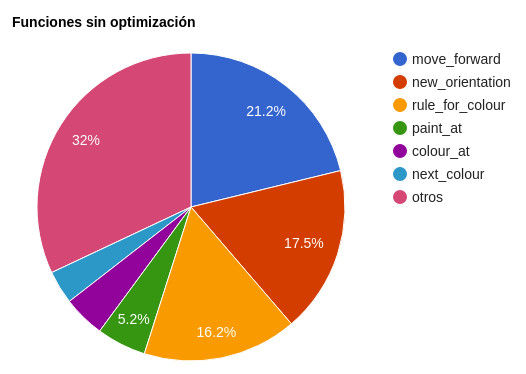
\includegraphics[scale=3]{chart.jpg} \\

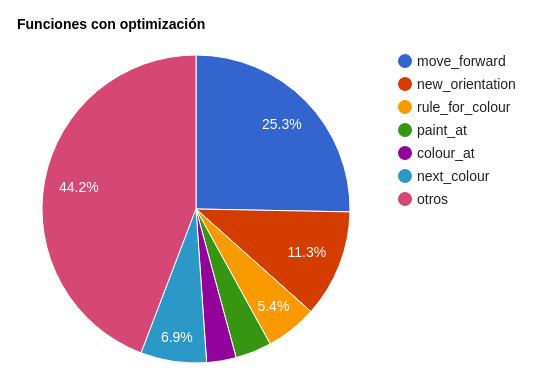
\includegraphics[scale=3]{chart2.jpg} \\

\begin{tabular}{|c|c|c|}
\hline 
Funcion & Tiempo(s): tp0\_if & Tiempo(s): tp0\_tables \\ 
\hline 
move\_forward & 95.8 & 115.2 \\ 
\hline 
new\_orientation & 79.1 & 51.1 \\ 
\hline 
rule\_for\_colour & 73.2 & 24.4 \\ 
\hline 
paint\_at & 23.5 & 17.1 \\ 
\hline 
colour\_at & 19.9 & 14 \\ 
\hline 
next\_colour & 15.8 & 31.2 \\ 
\hline 
\end{tabular} \\
 
 Calculamos los Speedup para las funciones llamadas dentro de la función \textbf{paint}:\\
 
\textbf{move\_forward}:
\begin{equation*} 
\begin{split}
 SpeedUp & =\frac{1}{(1-0.212) + \frac{0.212}{0.83}} \\
  &= 0.96
\end{split}
\end{equation*}

\textbf{new\_orientation}:
\begin{equation*} 
\begin{split}
 SpeedUp &=\frac{1}{(1-0.175) + \frac{0.175}{1.55}} \\
  &= 1.07
\end{split}
\end{equation*}

\textbf{rule\_for\_colour}:
\begin{equation*} 
\begin{split}
 SpeedUp &=\frac{1}{(1-0.162) + \frac{0.162}{3}} \\
  &= 1.12
\end{split}
\end{equation*}

\textbf{paint\_at}:
\begin{equation*} 
\begin{split}
 SpeedUp &=\frac{1}{(1-0.052) + \frac{0.052}{1.37}} \\
  &= 1.014
\end{split}
\end{equation*}

\textbf{colour\_at}:
\begin{equation*} 
\begin{split}
 SpeedUp &=\frac{1}{(1-0.044) + \frac{0.044}{1.42}} \\
  &= 1.013
\end{split}
\end{equation*}

\textbf{next\_colour}:
\begin{equation*} 
\begin{split}
 SpeedUp &=\frac{1}{(1-0.035) + \frac{0.035}{0.51}} \\
  &= 0.98
\end{split}
\end{equation*}

Teniendo en cuenta los seís módulos, el SpeedUp total calculado es de \textbf{1.026}.
\newpage

\section{Conclusión}

Si bien se esperaba tener una mejora en los tiempos de ejecución del programa no se lograron grandes mejoras, de hecho el programa en general tuvo una menor performance. Como se puede observar en los reportes para la misma cantidad de grillas e iteraciones(altas), los tiempos con la versión "mejorada" del programa fueron levemente mayores para todos los casos de prueba. Al incrementar la cantidad de grillas se logra un menor performance debido a la función \textbf{xalloc} que además de reservar el bloque de memoria, iniciliza el bloque. \\

La función \textbf{new\_orientation} mejora debido a que se usa un arreglo en vez de un \textbf{switch...case} que es menos eficiente, caso contrarion con la función \textbf{move\_forward} empeora debido a que se reemplaza un \textbf{switch...case} por un arreglo y agrega llamadas a funciones que a su vez estas agregan nuevas llamadas. La función \textbf{rule\_for\_color} presenta una leve mejora debido a que no se realiza una validación\textbf{(if...else)} como en la versión original.

La función \textbf{paint} mejora levemente, de acuerdo a los  cálculos un 2.6\%.




\vspace{.5cm}
%Referencias o recursos utilizados durante la investigación para la resolución del trabajo práctico 
\begin{thebibliography}{5}
 \bibitem{} La Universidad de Pensilvania.\\ \url{http://www.cse.psu.edu/~pdm12/cmpsc311-f16/}.
 \bibitem{} Profiling and Timing Code
.\\ \url{https://jakevdp.github.io/PythonDataScienceHandbook/01.07-timing-and-profiling.html}.
 \bibitem{} C to MIPS compiler
.\\ \url{http://reliant.colab.duke.edu/c2mips/}.
\end{thebibliography}
 

\end{document}
